\documentclass[10pt, letter]{article}

	\usepackage[margin=1in]{geometry}
	
	\usepackage[backend=bibtex, style=authoryear]{biblatex}
		
	\addbibresource{sources/sources.bib}
	\usepackage{hyperref}
	
			\title{\textsc{Neural Networks for Computed Tomography Imaging Spectroscopy of the Solar Atmosphere}}
			\date{\today}
			\author{Roy Smart \\ \url{roy.smart@montana.edu} \\ Montana State University, Department of Physics \\ Bozeman, MT 59717, USA}
			
	\usepackage{float}
	\usepackage{graphicx}
	\usepackage[font=scriptsize, labelfont=bf]{caption}
	\usepackage[font=scriptsize, labelfont=bf]{subcaption}
	
	\usepackage{wrapfig}
	
	\usepackage{pdfpages}


\begin{document}

	\maketitle
	
	\begin{abstract}
		
		Explosive events are a prominent feature in spectrographic observations of the solar transition region. A wide range of phenomena in the solar atmosphere have been found to be associated with explosive events, but are these really all examples of the same underlying mechanism, or are multiple mechanisms responsible for the spectral signature of explosive events? We propose to confront this question by performing snapshot imaging spectroscopy of the transition region. This measurement will provide cotemporal EUV emission line profiles over the full spatial extent of explosive events, permitting further characterization of these events through analysis of their spatial structure. A more complete understanding of the mechanisms responsible for explosive events is directly applicable to the NASA Heliophysics Division's objective of ``Exploring the physical processes in the space environment from the Sun to the Earth and throughout the solar system'' because the dynamics of explosive events are applicable to other regions of the solar atmosphere and may provide insight into long-standing questions about energy transport within the Sun.
		
		Snapshot imaging spectroscopy of the transition region will be achieved through computed tomography imaging spectroscopy (CTIS) of bright EUV emission lines. CTIS relies on the development of computed tomography algorithms to process data from such an instrument. To help answer the questions proposed above, we intend to develop a new algorithm for CTIS data analysis which is adapted to the environment of the transition region using neural networks. The development of such an algorithm will help to advance the method of CTIS and allow more complete investigations into the structure of the solar atmosphere.

		
	\end{abstract}
	
	\section{Problem Statement}	
	
		\subsection{Background} \label{back_sec} 
		
			The solar transition region (TR) forms the boundary between the dense, cool plasma of the chromosphere and the intense environment of the million-degree corona. It is through this region that the plasma composing the solar atmosphere undergoes a rapid temperature increase, rising from 20,000 K to 1 MK over a distance of just tens of kilometers. The processes through which energy is transmitted through this region and its influence on the rest of the solar atmosphere have remained the subject of considerable debate (\cite{Innes2015}).
			
			The dynamic environment of the TR is demonstrated by the observation of so-called explosive events (EEs), discovered by \cite{Brueckner1983} using the \textit{High-Resolution Telescope and Spectrograph} (HRTS) and further investigated by \cite{dere1989} and \cite{Dere1994}. Explosive events are spectral features present in TR emission lines, which are defined by non-Gaussian line profiles showing Doppler shifts between 50--150 km/s (\cite{Brueckner1983}). These events have been shown to occur on spatial scales of 2'' -- 5'', last approximately 600s (\cite{dere1989}), and are consistent with a bi-directional flow through the TR (\cite{Dere1991}; \cite{Innes1997}).
			
			While the properties of explosive events have been well studied, investigators have been unable to reach a consensus on the cause of these events. It has been postulated that EEs are the signature of siphon flows within small-scale loops (\cite{Teriaca2004}), flows along spicules and macrospicules (\cite{Wilhelm2000}), plasma ejection and retraction (\cite{Huang2014}), and evidence of magnetic reconnection through the plasmoid instability (\cite{Innes2015}). Furthermore, EEs have been associated with other events in the solar atmosphere such as coronal microflares (\cite{Krucker2000}), reconnection in the photosphere (\cite{Tarbell1999}), and the chromospheric jets observed by \cite{DePontieu2011}.
			
			While the literature describes a extensive list of properties and phenomena associated with explosive events, it remains unclear if all of these properties can be reproduced by a single mechanism, such as the plasmoid instability. From the wide variety of phenomena associated with explosive events listed above, it seems possible that a model of explosive events considering multiple mechanisms may be needed. \textbf{If these events do arise from multiple mechanisms, can we distinguish different types of explosive events by considering their spatial structure?}
			
			
			Measuring the spatial structure of explosive events relies on imaging spectroscopy, a technique that aims to spectrally resolve each pixel of an image. Unfortunately, the capabilities of current imaging spectrographs may be inadequate for a thorough exploration of explosive events. This is because current imaging spectrographs, such as the \textit{Interface Region Imaging Spectrograph} (IRIS) (\cite{De Pontieu2014}), can only view the sun through a thin slit, and must raster this slit across the sun to build up a spectrally-resolved image. This limited view prevents a complete characterization of explosive events, since only a small portion of the event can be observed at any one time.
			
			The limited observational capabilities of imaging spectroscopy through rastering have prompted the development of snapshot imaging spectroscopy (also known as snapshot hyperspectral imaging or simultaneous spectroscopic imaging), where every pixel in a scene is spectrally resolved in a single exposure. An observation of this type, if achieved using large spatial, spectral, and temporal resolution, allows the spectrum of an explosive event to measured across its entire spatial extent. A snapshot imaging spectroscopy technique known as computed tomography imaging spectroscopy (CTIS) (\cite{Okamoto:91}; \cite{bulygin:92}; \cite{Descour:95}) has been used by a mission known as MOSES developed by \cite{kankel1} to image the solar transition region. 
				
			 
		\subsection{Computed Tomography Imaging Spectroscopy}
			\label{inv_sec}
		
			Computed tomography imaging spectroscopy is an efficient method to perform snapshot imaging spectroscopy (\cite{kankel1}). It achieves this measurement by eliminating the slit of a conventional spectrograph, allowing a diffractive element to multiplex the spatial-spectral content of a scene into an image (\cite{Hagan2013}). This design is similar in spirit to observing a fireworks display through a diffracting pair of glasses; a scene observed by the detector will have its spectrum dispersed across the image in the outboard orders. To recover a spectrally-resolved image CTIS relies on forming mulitplexed images at multiple diffraction orders and using computational techniques to invert the mulitplexing operation and recover a spectrally-resolved image.
		
			Since a spectrally-resolved image can be represented by a 3D volume, we will refer to this sort of image as a spatial-spectral cube (SSC).  Computing this spatial spectral cube using images formed at multiple diffraction orders can be interpreted as a classic 3D tomography problem where $N$ projections are taken through a translucent 3D object in $x$, $y$ and $\lambda$ space (\cite{Bulygin:05}).
			\begin{wrapfigure}{R}{0.4\textwidth}
				\centering
				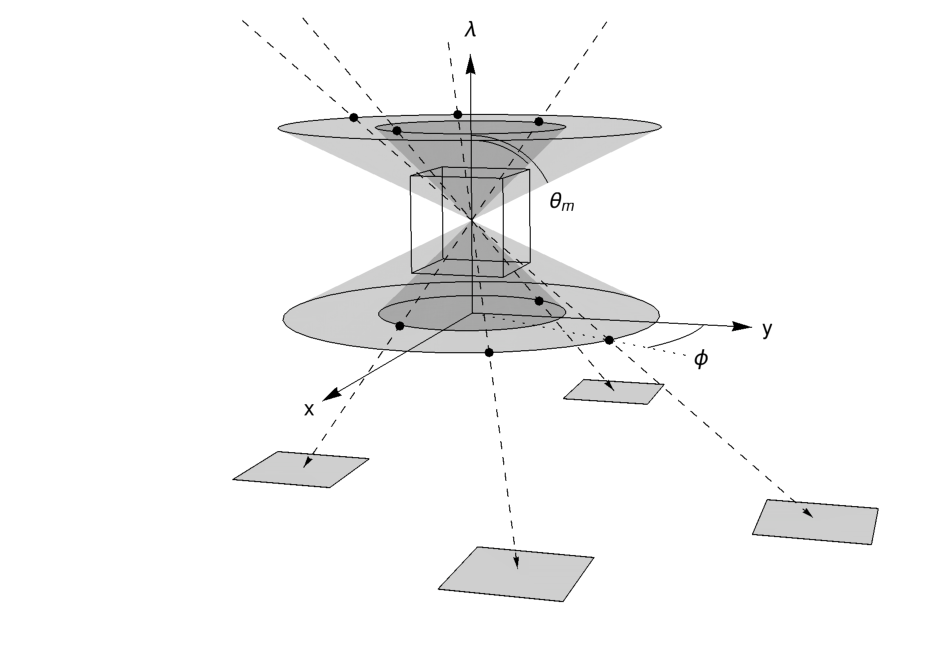
\includegraphics[width=0.4\textwidth]{figures/tomography}
				\caption{Geometry of the inversion problem for CTIS interpreted as a 3D tomography problem. $\theta_m$ describes the angle of the tomographic projection at each diffraction order and takes on discrete values, visualized by the nested cones. $\phi$ describes the dispersion direction and accepts continuous values. The four dotted lines are examples of particular projections through the spatial-spectal cube. Figure adapted from \cite{Bulygin:05}}
				\label{tomography}
			\end{wrapfigure}
			Using this representation, we can write the intensity in each order, $I_m$, of an object $v(x,y,\lambda)$ viewed by a computed tomography (CT) imaging spectrograph in terms of the intergral equation provided by \cite{fox1}
			\begin{equation}
				I_m (x',y') = \int_B v(x' - \lambda \tan \theta_m \cos \phi, \; y' - \lambda \tan \theta_m \sin \phi, \; \lambda) \; d\lambda,
				\label{tomo_eqn}
			\end{equation}
			where $x'$ and $y'$ are image coordinates and $B$ is the passband of the instrument. Equation \ref{tomo_eqn} is a Fredholm integral equation of the first kind (\cite{RHB}) with a projection kernel. Our goal is then to invert Equation \ref{tomo_eqn} to recover the object $v(x,y,\lambda)$. This problem will be referred to as the ``inversion problem'' or just simply an ``inversion'' for the remainder of this proposal.
			
			The CT imaging spectrographs developed by Charles Kankelborg and his research group only take between $N=3$ and $N=6$ projections through the spatial-spectral cube. This limited number of projections does not provide enough information to uniquely reconstruct the SSC, i.e. in the case of the CT imaging spectrographs discussed below (MOSES and ESIS), inverting Equation \ref{tomo_eqn} is an \textit{ill-posed problem} (\cite{inversion}). This means that there are multiple solutions to the inversion problem that satisfy a particular set of projections. To uniquely solve the inversion problem a CTIS inversion algorithm (CIA) must find a way to eliminate incorrect solutions to the inversion problem. We can show that many of the solutions to the inversion problem are unphysical, that is, they are inconsistent with physical law and previous solar observations.
			
			Therefore, an inversion algorithm must use physical constraints to trim possible solutions to the inversion problem and accurately reconstruct the spatial-spectral cube (\cite{inversion}). In Section \ref{pwork} we will briefly explore advantages and disadvantages of the physical constraints used by current inversion algorithms, and in Section \ref{prop_sol} we will propose to use machine learning algorithms to approximate these physical constraints and solve the inversion problem.
			
		\subsection{Current and Planned CT Imaging Spectrographs}

			In the sections below, we will conduct a limited overview of the current and planned CT imaging spectrographs designed and built by Charles Kankelborg and his research group. A brief understanding of the optical system of each instrument will be helpful to understanding the goals of this proposal. 

			Each of the instuments in the succeeding sections is designed to fly on a Black Brant IX sounding rocket launched from White Sands Missile Range. Additionally, each instrument is constructed with a narrow passband in EUV dominated by a bright emission line to alleviate intractability of the inversion process.

			\subsubsection{MOSES} \label{moses_intro}

				The Multi-Order Solar EUV Spectrograph (MOSES) has successfully undertaken two flights. The first flight occurred in 2005 and observed the Sun in He \textsc{ii} 304 \AA (\cite{fox1}) while the second flight was just recently completed in 2015 and observed the Sun in He \textsc{vii} 465 \AA (\cite{smart1}). 			
				 		
				\begin{figure}[h!]
					\centering
					\begin{subfigure}[t]{0.49\textwidth}
						\centering
						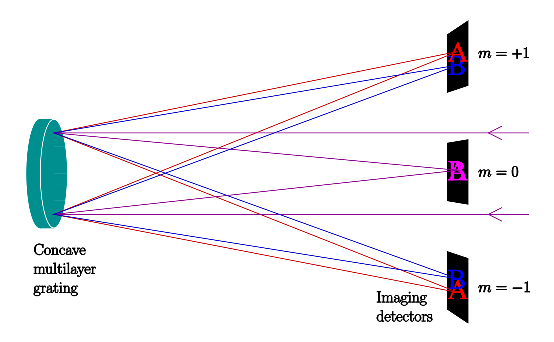
\includegraphics[height=2in]{figures/concave}
						\caption{Sketch of the optical system of MOSES}
						\label{optics}
					\end{subfigure}	
					~
					\begin{subfigure}[t]{0.49\textwidth}
						\centering
						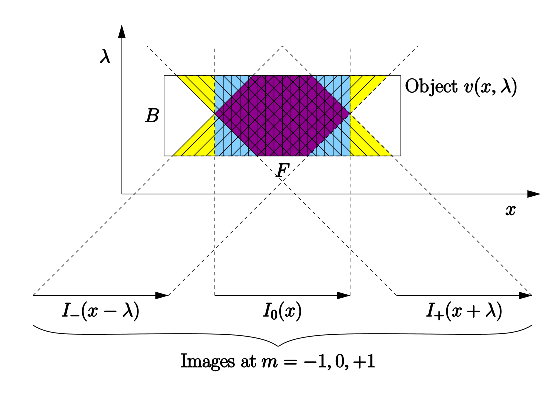
\includegraphics[height=2in]{figures/moses_cube}
						\caption{The analogue of Figure \ref{tomography} for the MOSES instrument.}
						\label{moses_tomo}
					\end{subfigure}	
					\caption{Two diagrams used to visualize the imaging system of the MOSES instrument. Figure \ref{optics} demonstrates how a bimodal spectral signal represented by a red `A' and a blue `B' are imaged by the MOSES optical system. Figure \ref{moses_tomo} imagines the MOSES optical system as a 2D tomographic projection through a spatial-spectral cube. Figures courtesy of \cite{fox1}}
				\end{figure}
				MOSES is a CT imaging spectrograph that uses a single concave diffraction grating to produce images in three spectral orders, $m=-1,0,1$, as in Figure \ref{optics} (\cite{kankel1}).
				This instrument is designed with dispersion in only one plane. Therefore, in the parlance of Figure \ref{tomography}, $\phi$ is restricted to the values of 0 and $\pi$ and then, without loss of generality, we can represent the 3D projections of Figure \ref{tomography} as 2D projections through a plane, as in Figure \ref{moses_tomo}.
				
				MOSES presents several challenges against achieving an accurate inversion. The most prevalent of these is the large astigmatism present in the outboard orders, which must be accommodated in any inversion process. 

			\subsubsection{ESIS} \label{esis_intro}
			
				The EUV Snapshot Imaging Spectrograph (ESIS) is the next generation of a CT imaging spectrograph developed by Kankelborg and his research group. This instrument will be equipped with one large focusing primary mirror, and small, dedicated diffraction gratings for each detector. The first flight is planned for 2019 and the instrument will be equipped with four detectors to image the $m=1$ order in four separate dispersion directions. After the first flight has been completed, the system will undergo upgrades to install two additional gratings and detectors for a total of six tomographic projections. 
				
				The tomographic projections of the ESIS instrument can be visualized in terms of Figure 1. The dedicated diffraction gratings are arranged in an octagonal pattern, producing projections at $\phi = 0$, $\pi/8$, $\pi/4$, $3 \pi / 8$, $\pi /2$, $5 \pi /8$, and $3 \pi /4$. Since these projections are not all in the same plane (unlike the MOSES arrangement), the inversion problem cannot be reduced to two dimensions and must be solved in 3D.
			
		\subsection{Related Work} \label{pwork}
		
					\begin{wrapfigure}{R}{0.2\textwidth}
						\centering
							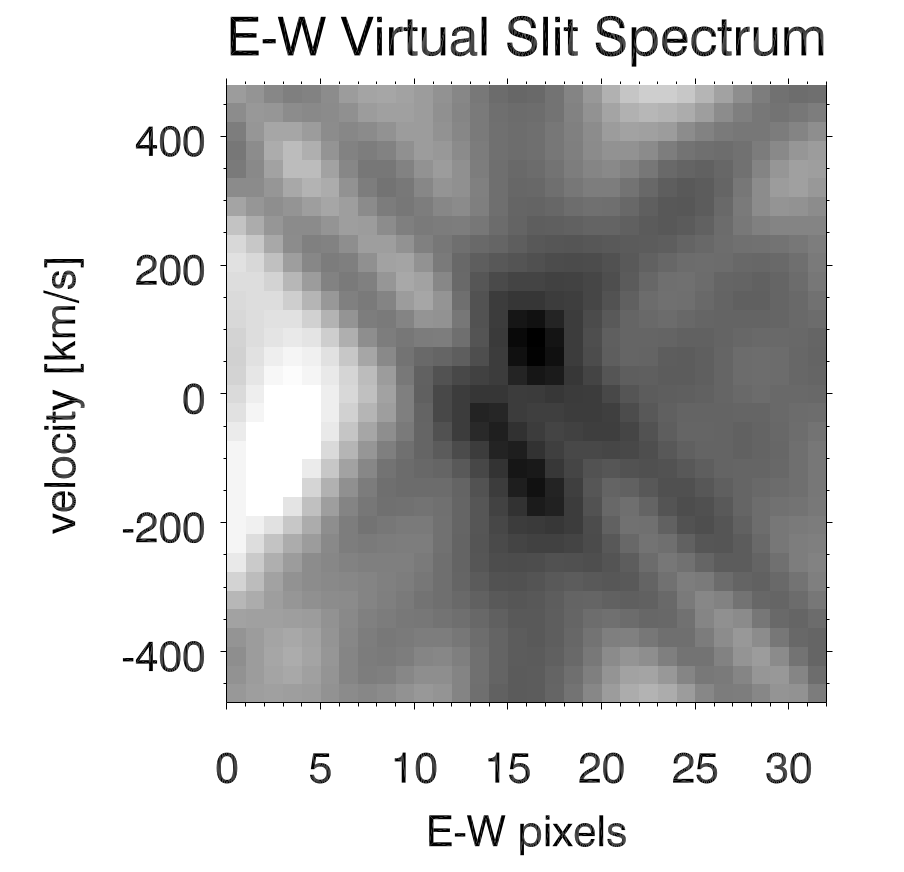
\includegraphics[width=0.2\textwidth]{figures/plaid}
						\caption{An example of plaid produced by SMART. The vertical dimension is the spectral dimension in units of relative doppler shift from line center, and the horizontal axis is position measured in pixels. Image courtesy of Thomas Rust.}
						\label{plaid}
					\end{wrapfigure}
			
			The task of inverting MOSES data has already been undertaken by several research projects (\cite{inversion}; \cite{fox1}). The most effective inversion algorithm developed by these efforts is known as the \textit{smooth multiplicative algebraic reconstruction technique} (SMART) developed by \cite{kankel2} based off of earlier algebraic reconstruction techniques invented by \cite{Gordon70} and refined by \cite{Okamoto:91}. As discussed in Section \ref{inv_sec}, any CTIS inversion algorithm must use physical constraints to find unique solutions. In the case of SMART, it uses the property that its solutions to the inversion problem must satisfy positivity and definitions of average line profiles to enforce physicality.
						
			The result is a very efficient algorithm that has been successfully used to determine doppler shifts and line profiles of explosive events in He \textsc{ii} (\cite{rust1}).
			Unfortunately, it has proven difficult to convince SMART to produce physical inversions across the entire MOSES dataset. This unphysicality is mainly produced by an artifacts known colloquially as \textit{plaid}. As an example, in Figure \ref{plaid} we can see that the bright object in the center has been blurred at the angles: $\theta=-\pi/4$, 0, and $\pi/4$ (with respect to the vertical) resulting in plaid. 
					
			Plaid occurs whenever SMART attempts to invert a set of CTIS images with a background signal. Therefore, to yield plausible results using SMART, the background must be manually subtracted to isolate and successfully invert the area of interest. This operation prevents the creation of an automated, global inversion process for MOSES data.

		\subsection{Project Goals}
		
			Snapshot imaging spectroscopy using CTIS is a promising method for resolving the spatial-spectral structure of explosive events. However, data analysis for these types of instruments is a challenging problem.
			Therefore, to approach our goal of determining the spatial structure of explosive events, we propose to conduct this investigation in two phases. In the first phase, we will develop a new algorithm to solve the inversion problem using neural networks. Our goals for this algorithm are speed and supression of plaid artifacts. During the second phase, we will apply our inversion techniques to MOSES and ESIS to explore the spatial scale of explosive events. The remainder of this proposal will be devoted to a discussion of the first phase due to space constraints. We hope to further develop ideas for analyzing the spatial-spectral cubes produced by MOSES and ESIS in later proposals. 
		
	\section{Proposed Solution} \label{prop_sol}
	
		So far, all CIAs have utilized physical constraints derived from first principles (such as positivity). This is not the only way however, instead an inversion algorithm could build physicality constraints based off of direct observation of the solar spectrum. For example, IRIS has been measuring the spectrum of the Sun since 2013 (\cite{De Pontieu2014}), and has amassed a large dataset composed of observations of the solar spectrum. An inversion algorithm that incorporates these observations has the potential to calculate inversions with greater accuracy because it has an appreciation for typical structures seen in solar EUV emission lines.
		
		One possible way to appy a set of solar spectroscopic observations to an algorithm is by using machine learning. Machine learning is a problem solving technique that allows a computer to learn a relationship between a set of problems and their associated solutions. Artificial Neural Networks (ANNs) are possibly the most popular type of machine learning algorithms, and they have been used successfully to solve a wide variety of problems such as classification, function approximation, and data compression. Recently, it has been shown that ANNs have the capability to solve problems critical to solar data analysis such as denoising (\cite{DAEC}) and PSF deconvolution (\cite{nn_psf}). ANNs have even been successful in solving ill-posed problems (\cite{Kruglov2013}), inversion problems (\cite{Jafarian2015}) and computed tomography problems (\cite{Boublil2015}). Due to the success of ANNs at solving these types of problems we hypothesize that a CIA represented by a neural network and trained using real solar spectroscopic data would be able to form reasonable solutions to the inversion problem.
		
		\subsection{A Brief Introduction to Neural Networks}
		
			For the purposes of this proposal, we will view the neural network as a black box, with the capability to approximate any function (\cite{ai}). Neural networks can approximate any function, if they are provided enough free parameters known as \textit{weights}. These weights are learned through a process known as training, where a neural network is presented with a large number of example inputs to the function to be approximated. The network is then asked to compute the value of the function, and it is given feedbaack based on the error between its value and a known value. Algorithms are used to minimize the error by adjusting the weights of the network.
		
		\subsection{Inversion Using Neural Networks}
		
			With the basic description provided in the previous section, we can begin to discuss how we one would build a CIA using neural networks, which we will call a \textit{CTIS inversion neural network} (CINN). To summarize Section \ref{inv_sec}, a CIA solves a computed tomography problem, which reconstructs a 3D object using a set of 2D projections. Thus, a CINN's input layer will be a set of neurons representing each pixel in each 2D projection and a CINN's output layer will be a set of neurons representing each voxel of the SSC. These layers will be connected by an unknown number neurons to be determined during training. 
					
			To create the training dataset, we start by constructing a spatial-spectral model of the Sun. Since MOSES and ESIS are designed with a narrow passband, the spectral range of this model need not be immense, but it should be representative of the Sun as observed by MOSES and ESIS. As indicated above, this model will be composed of direct spectroscopic observations of the Sun from existing instruments. However, there are no spectrographs that observe the Sun in the same passband as ESIS and MOSES, so we will use observations of emission lines with comparable formation temperatures to that of the emission lines in the passband of MOSES and ESIS. 
			
			This spatial-spectral model forms what we will call the ``truth dataset''. From the truth dataset, we will generate the ``input dataset'' by using a forward model of the optical system of each instrument. MOSES and ESIS have different optical systems, so to solve the inversion problem for each instrument, we will be required to train two neural networks. The input and truth datasets taken together form the training dataset. During training, data from the input set will be fed into the CINN, and data from the truth dataset will be compared to the output of the CINN to direct the learning process.
			
			\subsubsection{MOSES Inversion} \label{moses_inv}
			
				MOSES is the simplest instrument to implement a CINN because it can be represented as a 2D tomography problem (Section \ref{moses_intro}). As such, the training data for MOSES may be constructed out of simple slices of the SSC. Using the Si \textsc{iv} 1403 \AA\ IRIS dataset to construct the truth dataset for this instrument is an obvious choice, as both the Si \textsc{iv} 1403 \AA\ and He \textsc{ii} 304 \AA\ are both low transition region lines, and we simply want to inform our network of common features seen in these lines.
		
			
			\subsubsection{ESIS Inversion}
			
				Unlike MOSES, recovering the SSC from ESIS data requires a 3D solution to the inversion problem (Section \ref{esis_intro}). Therefore, the truth dataset of an ESIS CINN takes the form of an array of SSCs, which are most easily acquired by using IRIS in raster mode. Unfortunately, few of the rasters produced by IRIS are taken at a high enough spatial resolution to provide a realistic SSCs, and we will need a large number of SSCs to effectively train a CINN. There are several approaches to circumventing this problem, the easiest of which is to naively stacking spectral images to form a psuedo-realistic SSC to be inserted into the truth dataset. 
		
		\subsection{Preliminary Results}
		
			To test if a CINN could be a useful inversion tool, we trained a CINN to invert a simplified forward model of MOSES. This CINN used a input dataset that did not incorporate elements of the MOSES forward model such as the PSF, shot noise or readout noise. While this simplification is certainly unrealistic, this CINN serves to illustrate a proof-of-concept and to justify additional research into this method.
			
			This CINN was trained using approximately 500k truth images with a size of $21 \times 21$ pixels. These images were extracted from the IRIS Si \textsc{iv} 1403 \AA{} dataset, and were background subtracted to further simplify the inversion problem for this test. This CINN was trained on an Nvidia 980 consumer GPU using the Caffe (\cite{jia2014caffe}) neural network library. 
			
			\begin{figure}[h!]
				\centering
				\begin{subfigure}[t]{0.1\textwidth}
					\centering
					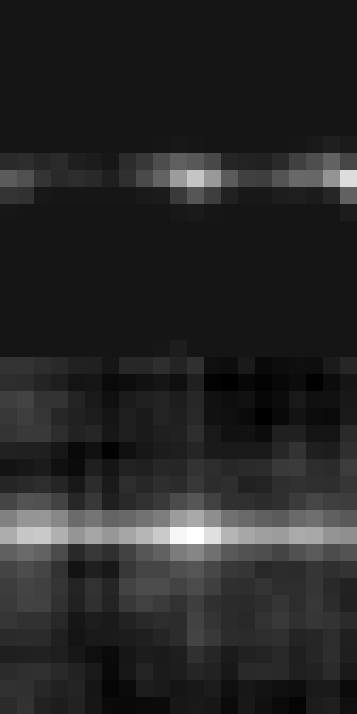
\includegraphics[width=\textwidth]{figures/inv1}
				\end{subfigure}	
				~
				\begin{subfigure}[t]{0.1\textwidth}
					\centering
					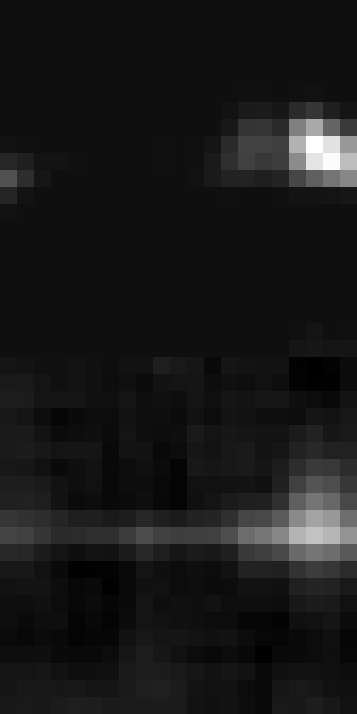
\includegraphics[width=\textwidth]{figures/inv2}
				\end{subfigure}	
				~
				\begin{subfigure}[t]{0.1\textwidth}
					\centering
					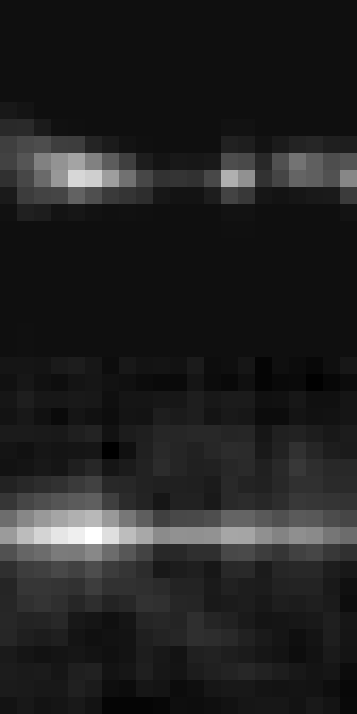
\includegraphics[width=\textwidth]{figures/inv3}
				\end{subfigure}	
				~
				\begin{subfigure}[t]{0.1\textwidth}
					\centering
					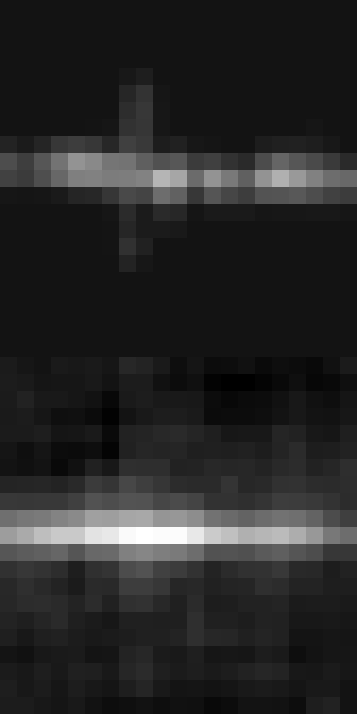
\includegraphics[width=\textwidth]{figures/inv4}
				\end{subfigure}	
				~
				\begin{subfigure}[t]{0.1\textwidth}
					\centering
					
\includegraphics[width=\textwidth]{figures/inv5}
				\end{subfigure}	
				\caption{A visualization of the inversions produced by a simple implementation of a MOSES CINN. The top image is the truth image and the bottom images is the output of the CINN.}
			\end{figure}	
			
			This test provides exciting verification to the efficacy of this method. The quality of the inversions show that the neural network is learning concepts such as: line center, mean line width and the correct distribution of intensity through the inversion. We can see that this neural network isn't always able to produce the exact line profiles of the more energetic events, and often overestimates the intensity of the line core. We hope to train later neural networks with much more data, and many more neurons, allowing the creation of more accurate CINNs.
		
	\section{Relevance to Heliophysics}
	
		The NASA Heliophysics Division has the goal of ``Explore the physical processes in the space environment from the Sun to the Earth and throughout the solar system''. We believe that the study of transition region explosive events fulfills the desired intent of that goal because these explosive events are thought to be direct evidence of reconnection. Reconnection is thought to be an important process in the dynamics of the solar atmosphere and further insight into these processes has many wide-reaching implications for heliophysics.
	
	\section{Project Timeline}
		The schedule for the first year of this proposal is described by the figure below.
		\begin{figure}[h!]
			\centering
			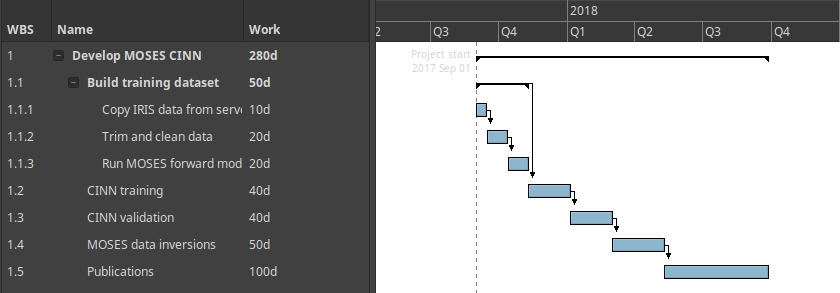
\includegraphics[width=0.8\textwidth]{figures/schedule}
		\end{figure}
		
		We propose to use the CINN developed during the first year of this proposal to perform data analysis on data from ESIS, MOSES and orbital spacecraft during subsequent years. Defining a schedule for the last two years of this proposal is difficult due to the tenuous nature of spaceflight using sounding rockets. Therefore, we intend for the schedule of the second phase of this proposal to be the discussion of future proposals.

	\printbibliography

	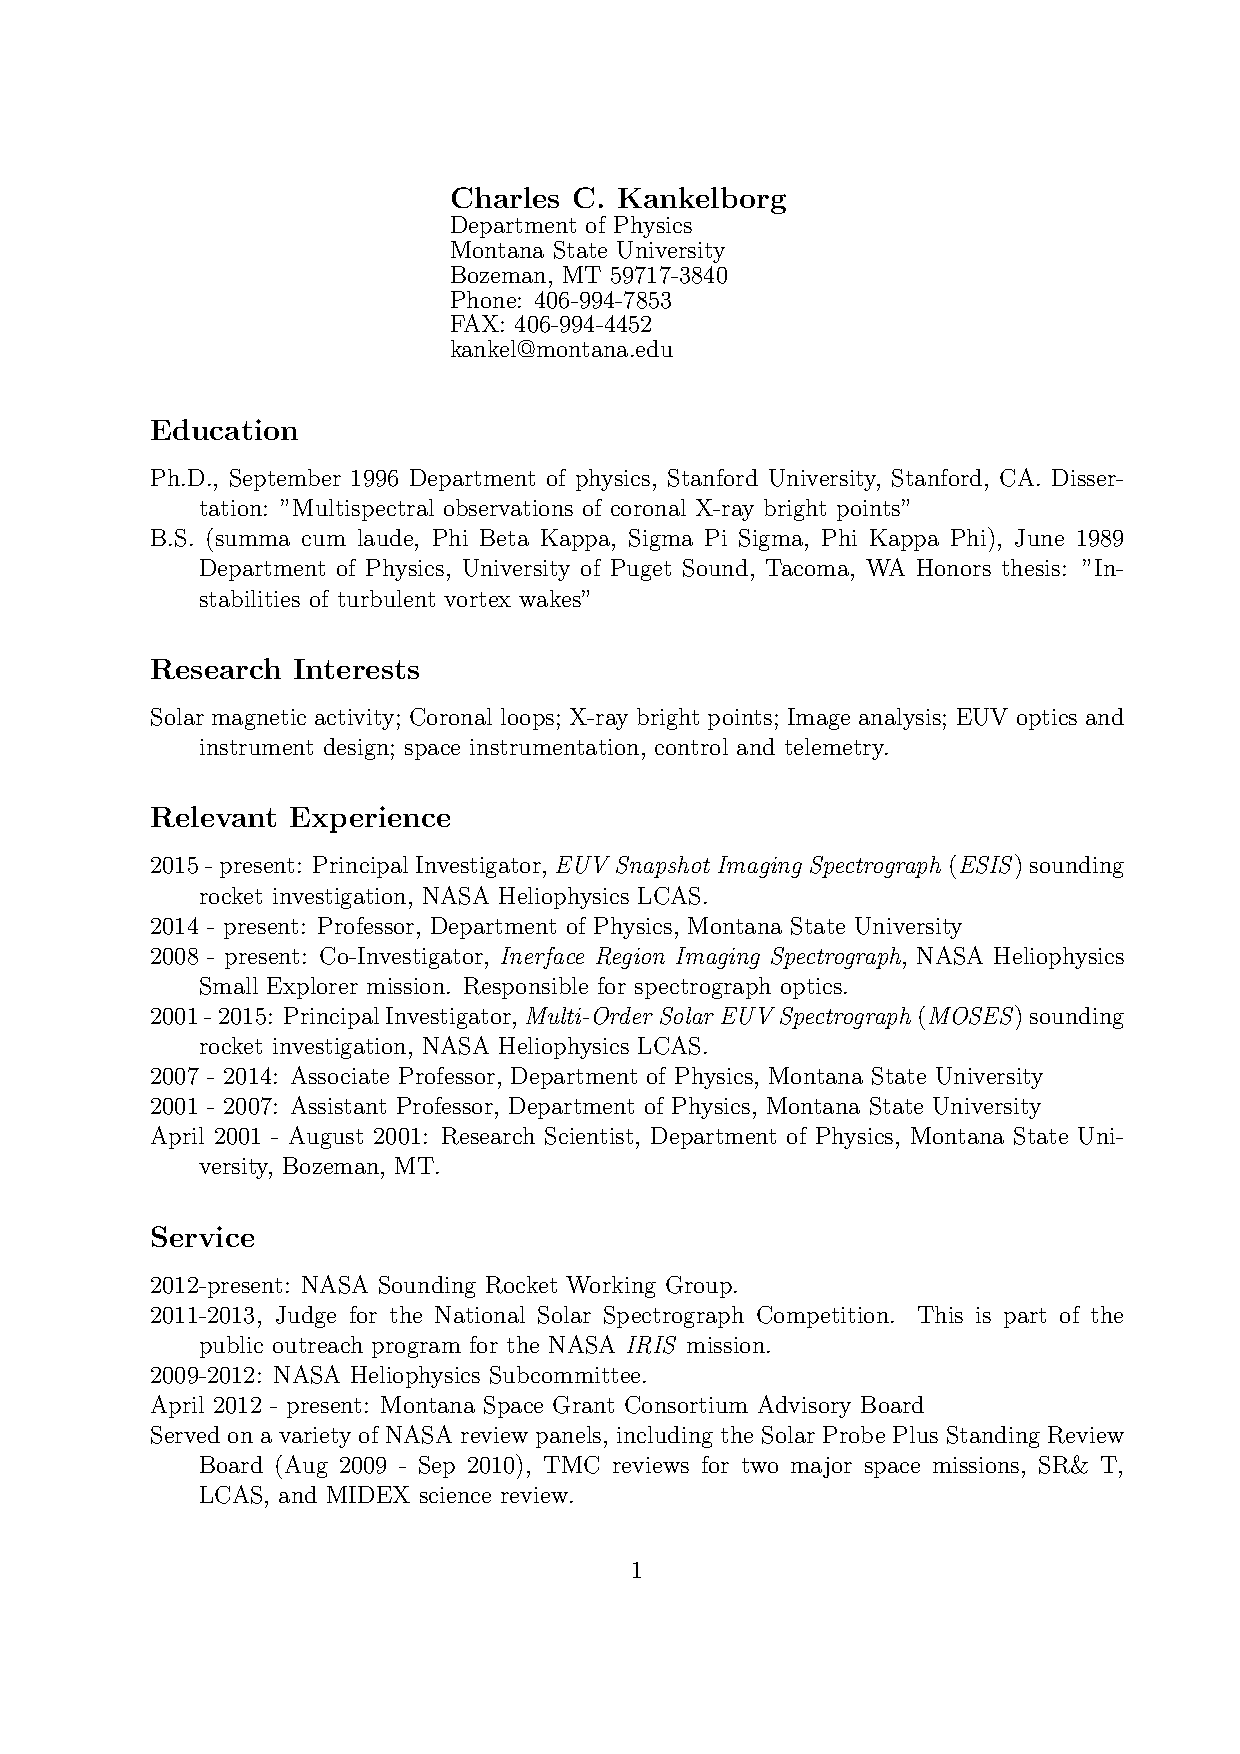
\includepdf[pages=-]{cv4ck_2p}
	
\includepdf[pages=-]{royCV}
	
\includepdf[pages=-]{nessf17smartLetter}
	
\includepdf[pages=-]{NESS17_smart_affirmation}
	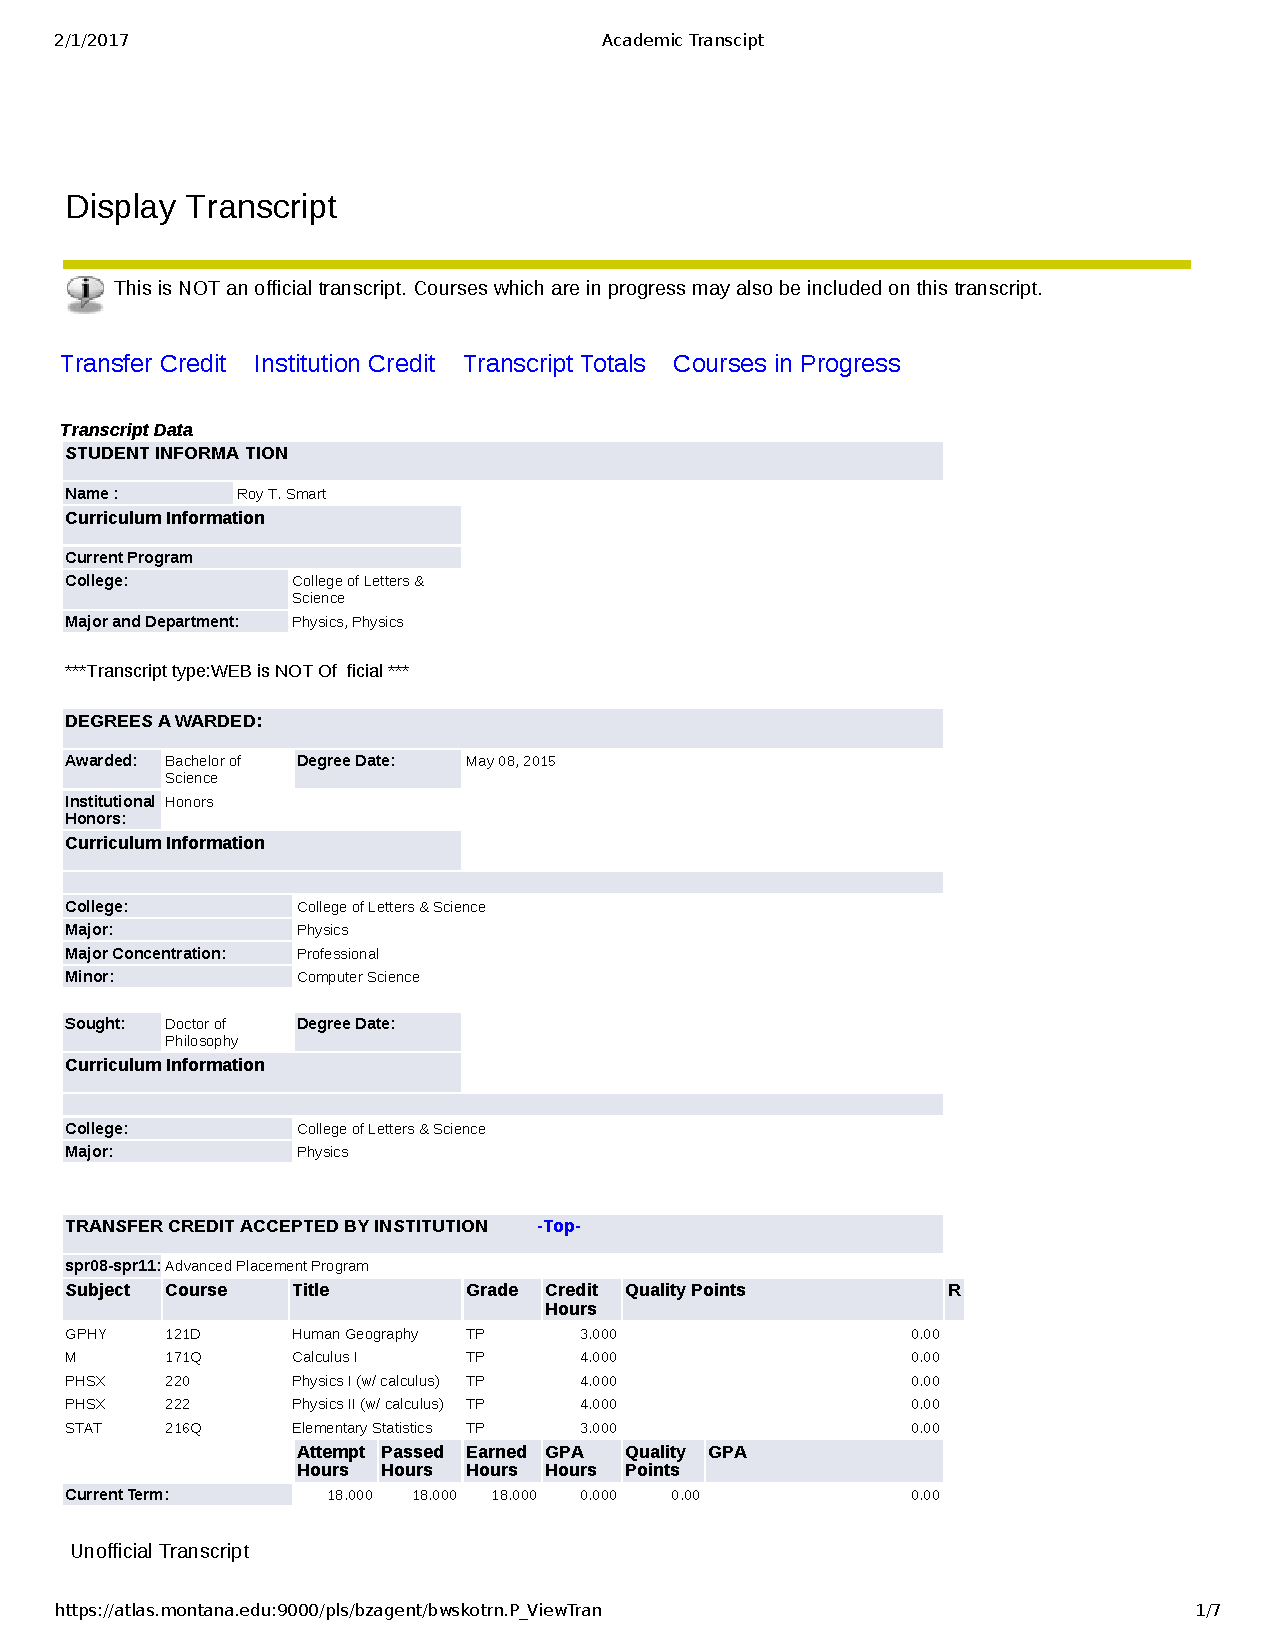
\includepdf[pages=-]{transcript}
	
	
\end{document}

